\documentclass[11pt]{article}

\usepackage{amsmath}
\usepackage{textcomp}
\usepackage{tikz}
\usepackage[top=0.8in, bottom=0.8in, left=0.8in, right=0.8in]{geometry}
% add other packages here

% put your group number and names in the author field
\title{\bf Exercise 2: A Reactive Agent for the Pickup and Delivery Problem}
\author{Group \textnumero 17: Ogier Bouvier, Val\'erian Rousset}

% the report should not be longer than 3 pages

\begin{document}
\maketitle

\section{Problem Representation}

\subsection{Representation Description}
% describe how you design the state representation, the possible actions, the reward table and the probability transition table

The state is an object containing the 3 following informations.

First we have the current city the agent is in. The second property is
a boolean indicating whether the agent is currently performing a task
and the last one is the destination city if the agent carries a task
or nothing otherwise.

From each of these state we have two possibilities

\begin{itemize}
	\item If we have a task, move to the destination city.
	\item If we don't have a task, we go to the neighbooring city which
		has the best potential reward, the reward of a package minus
		the cost of travelling there. Cost itself is defined by the
		distance to the city times the cost per kilometer.
\end{itemize}

\subsection{Implementation Details}
% describe the implementation details of the representations above and the implementation details of the reinforcement learning algorithm you implemented

For each possible state, we find the possible actions (for exemple, we can't
deliver if we don't have a task), then for each, we compute the best
reward weighted by the probability of  and add it to the generated
map. Then, we do it over and over (for each path in the state graph),
until the map stabilize, meaning that we have reached the optimal
value for every state.

Invalid actions will never be performed by the agent since all actions
are checked before being added to the state transition map.

\section{Results}
% in this section, you describe several results from the experiments with your reactive agent

\subsection{Experiment 1: Discount factor}
% the purpose of this experiment is to understand how the discount factor influences the result

\subsubsection{Setting}
We tested using three different discount factor. One agent runs with a
discount factor of 0.20, another 0.60 and the last 0.90.

The experience can be repeated by running the simulation with
reactive-rla20, reactive-rla60 and reactive-rla90 agents.

\subsubsection{Observations}
\begin{figure}
  \caption{Simulation result for the three different settings}
  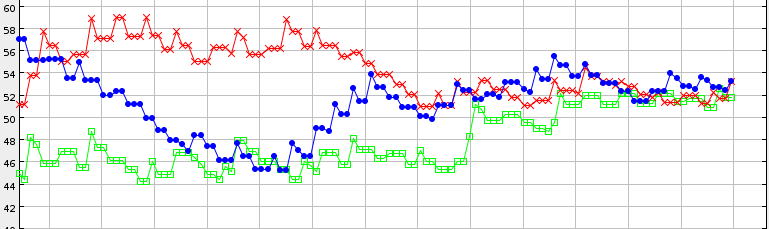
\includegraphics[scale=0.7]{compare_discount}
  \centering
\end{figure}

We fail to see a clear difference between the 3 settings of discount
factor, except maybe the fact that the blue agent seems to stabilize
its average reward faster than the other two leading us to think that
the higher the discount factor, the faster the agent stabilizes its
average reward per kilometer.

\subsection{Experiment 2: Comparisons with dummy agents}
% you compare the results of your agent with two dummy agents: the random agent that was already given in the starter files and another dummy agent that you define and create. You should report the results from the simulations using the topologies given in the starter files and optionally, additional topologies that you create.

\subsubsection{Setting}
We have implemented a dumb agent which is basically the same as the
Random agent except it always picks up task when one is available. If
not it will move to random neighbor of the current city.

We run all 3 agents in one simulation. The first two have a discount
factor of 0.85 and the second one has no parameter.

\subsubsection{Observations}
\begin{figure}
  \caption{Simulation result for the 3 agents comparison}
  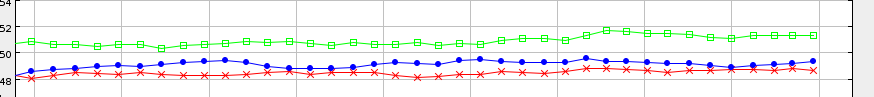
\includegraphics[scale=0.6]{compare_3}
\end{figure}

We notice that our agent performs clearly better than the other two
(about 200 more reward per kilometer), while the dumb agent perform
almost the same as the random agent.


\end{document}
